\documentclass[acmsmall]{acmart}

\usepackage{graphicx}
\usepackage{amsmath}
\usepackage{booktabs}
\usepackage{hyperref}
\usepackage{float}

% Configure graphics path based on the zip folder structure
\graphicspath{{../results/Figures/}}

\begin{document}

\title{An Empirical Audit of Automated Metrics for Epistemic Preservation in LLM-Assisted Editing}
\author{Yuvraj Singh Rajawat}
\affiliation{%
  \institution{Center for Artificial Intelligence in Scientific Communication, IIIT Allahabad}
  \city{Prayagraj}
  \country{India}
}
\email{PHM2026001@iiita.ac.in}

\begin{abstract}
Assessing Large Language Models (LLMs) for scientific editing requires metrics that can tell when claims have been rephrased without changing their meaning. Due to the probabilistic nature of LLMs, claims often undergo parametric memory override in which critical epistemic hedging is lost and replaced with assertive causal statements. In this work, we propose an asymmetric Natural Language Inference (NLI) divergence metric ($\Delta_{\text{epistemic}}$) to measure directional epistemic overrides using a bespoke test set of 200 biomedical claim pairs. Our main hypothesis was falsified; General domain NLI cross encoders were unable to differentiate between different types of causality overrides (ROC-AUC=0.3234) and treated verb category overrides as contradictory. Explicit prompting using generative LLMs to utilise taxonomic overrides resulted in high context overloading and synonym creation (ROC-AUC=0.6002). We found that BERTScore, a measure of deep context embedding differences inherently and reliably identifies causality overrides under fixed context minimal-pair conditions (ROC-AUC=0.9518). We conclude that semantic distance measurements provide a superior method to logical entailment, with zero-shot methods, to audit epistemic overrides in AI edited text.
\end{abstract}

\maketitle

\section{Introduction}

With the rise of Large Language Models (LLMs), there has been a huge change in academic writing. Scientists are using AI tools to help them at all stages of the writing process, from initial drafts to developmental editing. While it is clear that LLMs can improve the syntax, it is unclear how they affect the semantics of the text such as accurate representation of the science.
 
There are two purposes of scientific writing. Firstly, accurately describing what has been observed. Secondly, determining just how much evidence there is to support a wider explanation of a phenomenon. Whether or not a relationship is statistical or causal is an important aspect of the research itself. After many years of training researchers will use precise and cautious wording (e.g. associated with, linked to) in their writing to accurately represent the limitations of data from observations. They will avoid words that imply causality (e.g. causes, determines) unless they have a very tightly controlled experimental design.

However, the models are constantly changing meaning. If the model is asked to improve ``flow'' or ``readability'', it will make modifications based on correlations it observed during training, which we hypothesize may stem from training data distributions favoring authoritative language. This correlation to causation algorithm can cause problems by introducing scientific ``spin''. This can mislead the reader. \cite{chiu2017spin}.

In this paper we aim to address this issue. We introduce and evaluate a novel asymmetric Natural Language Inference (NLI) metric ($\Delta_{\text{epistemic}}$). Through a meta-evaluation of 200 biomedical claims, we investigate how we can better maintain the causal boundaries in text using either a similarity between continuous embeddings or through zero shot logical entailment.

\section{Theoretical Foundations and Related Work}

\subsection{The Epistemology of Causal Inference}

To understand the severity of the semantics-changing effect we must first consider the underlying epistemological principles. In particular, Pearl's ``Ladder of Causation'' \cite{pearl2018book} defines what it means to infer causality. We can represent the key distinction between observation and causation:

\begin{equation}
P(Y=y \mid X=x) \neq P(Y=y \mid do(X=x))
\end{equation}

By saying "A is associated with B", the author is claiming $P(Y \mid X)$. However, if the LLM changes this sentence to "A causes B" to sound more authoritative then the LLM is increasing the claim to $P(Y \mid do(X))$ and changing the scientific truth of the text \cite{hernan2020causal}.

\subsection{The Psycholinguistics of Scientific Reading}

This is worsened by human cognitive biases. Gershman and Ullman \cite{gershman2023causal} have shown that humans often infer causality in purely correlational claims. Even if researchers carefully phrase their claims using very cautious and well-known phrasing, lay people---and even trained experts---often mentally interpret this as causal statements. Thus, the removal of language friction (caused by hedging and caveats) in LLMs greatly exacerbates this natural bias towards causal thinking.


\subsection{Technical Mechanisms of Semantic Distortion}

Understanding why advanced LLMs fail to preserve causal language requires analyzing their underlying architectures. 

\begin{itemize}
    \item \textbf{Parametric Memory Override \& Constraint Poisoning:} Latif \cite{latif2026constraint} noted that LLMs often disregarded constraints provided by users (e.g., ``do not use causal verbs''), and instead rely upon the weighted distribution of training data. The model confuses the frequent occurrence of strong causal language throughout the training set with truth in science within the manuscript. This is known as constraint poisoning.
    \item \textbf{Absence of Structural Causal Models:} LLMs have no inherent causal reasoning capabilities. Fu et al. \cite{fu2025correlation} found that LLMs are purely working with high dimensional correlations, they have no actual understanding of the causal, physical/timing processes between variables. 
\end{itemize}

This means LLMs are essentially highly complex causal parrots. Therefore there is an urgent need for them to be audited automatically.

\subsection{Computational Detection of Causal Claim Strength}
Identifying and evaluating causality claims computationally has developed significantly. Previous work used manually annotated data to identify and classify high-level categories of causal relationships such as correlational, conditional cause and direct cause relationships \cite{sumner2014association}. This was later automated by using domain specific BERT models fine-tuned for the task on multi-domain data from PubMed abstracts and EurekAlert! press releases \cite{yu2019detecting, yu2020measuring}.

Recent work has focused on zero-shot evaluations of Large Language Models. It has been shown that models such as ChatGPT will understand causal language when prompted explicitly but will not perform well with hedging and conditional claims \cite{kim2023chatgpt}. The previous work uses a sentence level approach to classify causality as a discrete text classification task. Our work introduces a new method of pairwise shift detection. We calculate the continuous epistemic divergence ($\Delta_{\text{epistemic}}$) between the original and modified sentences. This allows us to evaluate how much change there is in the meaning of the sentences with LLMs.

\section{Taxonomy of Epistemic Shifts}

Based on our observations of editing in LLMs, we focus on the most dangerous category in our taxonomy of AI induced semantic distortion: \textbf{Causal Escalation} which occurs when a model strengthens the strength of a claim within an evidence by:

\begin{enumerate}
    \item \textit{Correlational to Causal Shift:} Changing a verb explicitly from correlation to causation (e.g. editing ``Coffee consumption is associated with lower heart rate'' to ``Coffee consumption lowers heart rate'').
    \item \textit{Removal of Epistemic Hedges:} Removing hesitation words due to training under RLHF.
\end{enumerate}

\section{Methodology}

\subsection{Diagnostic Dataset Formulation}

We developed our own diagnostic tests (\texttt{custom\_epistemic\_suite.csv}). The base claims were extracted from the PubMed database using the NCBI Entrez API. We filtered claims to only include those with the terms 'observational study' or 'cohort' in their metadata and containing correlation keywords (e.g. 'associated with', 'correlated with', 'linked to') in their text.

We used a generative large language model (ChatGPT) to extend these claims into evaluation triplets. By carefully designing prompts, we were able to limit ChatGPT's role to that of a biomedical linguistics expert. We used the model to create two variations of each claim.
\begin{enumerate}
    \item \textbf{Semantic-Preserving Paraphrase (Negative Control, label 0):} A sentence that is rewritten for syntactic and lexical variation but retains the original epistemic information.
    \item \textbf{Unwarranted Causal Escalation (Test Case, Label 1):} Rewritten sentences that change the correlational verb to a causal verb (e.g., causes, prevents, results).
\end{enumerate}
Importantly, this generation template specifically prevented the introduction or removal of any biomedical entities, populations or statistical directionality ensuring only the epistemic verb transformation would be performed. This resulted in the creation of 100 perfectly balanced triplets creating 200 comparison examples (original, paraphrased).

During quality control validation, we identified 3 triplets (P019, P060, P093) that were not transformed by the generative LLM resulting in duplicate strings. These were manually corrected to ensure our ground truth labels reflect the presence of any epistemic transformation. This data set provides a lexical benchmark with minimal pair transformations within a fixed context. It is not a syntactic paraphrasing task.

\subsection{Baseline and Proposed Metrics}

The evaluation was performed using three typical symmetric evaluation methods based on lexical (BLEU \cite{papineni2002bleu} and ROUGE-L \cite{lin2004rouge}) and deep semantic similarity (BERTScore \cite{zhang2019bertscore} via \texttt{microsoft/deberta-xlarge-mnli} \cite{he2021deberta}).

To capture the logical dependency between scientific statements, we propose an asymmetric Natural Language Inference (NLI) based divergence metric $\Delta_{\text{epistemic}}$. This means that causal statements can be inferred from correlational ones, however not vice versa. Formally we define:

\begin{equation}
\Delta_{\text{epistemic}} = P_{\text{entail}}(S_{\text{orig}} \mid S_{\text{edit}}) - P_{\text{entail}}(S_{\text{edit}} \mid S_{\text{orig}})
\end{equation}

\subsection{Targeted Theoretical Modification: Generative LLM (Pathway C)}

We initially computed $\Delta_{\text{epistemic}}$ with a zero-shot cross-encoder (\texttt{cross-encoder/nli-deberta-v3-large}). As we observed it failed to represent the causal taxonomic structure, we designed a targeted hypothesis (\textit{ Pathway C }). We replaced the cross encoder with a quantized generation LLM with local knowledge (\texttt{Qwen2.5-1.5B-Instruct}). 

During evaluation, the LLM was given a highly constrained zero shot prompt including the precise structure of the epistemic hierarchy:

\begin{quote}
``\textbf{Premise}: \{premise\_text\} \\
\textbf{Hypothesis}: \{hypothesis\_text\} \\
\textbf{Rule 1}: A correlational finding (e.g., `associated with') does NOT entail a causal finding. \\
\textbf{Rule 2}: A causal finding (e.g., `causes', `contributes to') logically ENTAILS a correlational finding. \\
\textbf{Task}: Based strictly on these rules, what is the probability (from 0.0 to 1.0) that the Premise entails the Hypothesis? Output only the numeric float.''
\end{quote}

This manipulation was implemented by adding explicit information about how to use taxonomy during the prompt construction. As the model produces text responses, we used a regular expression parser (\texttt{r"0\.\textbackslash d+|1\.0|0"}) to extract the float value. If any exception occurred while extracting the float value, the neutral value of 0.5 was used.

\section{Experimental Setup}

All experiments were carried out using the Tesla T4 GPU (15GB VRAM) with PyTorch 2.14 and Python 3.13. All environments were seeded deterministically (Seed=42). The LLMs were decoded using greedy search only (\texttt{do\_sample=False}). The NLI tokenizers were initialized with \texttt{use\_fast=False}.

The Receiver Operating Characteristic Area Under the Curve (ROC-AUC) and Spearman's rank correlation ($\rho$) was calculated to measure how well each metric discriminates between paraphrased and escalated edits. 95\% Confidence Intervals were calculated using 2000 non-parametric bootstrap samples. Because BERTScore, ROUGE, and BLEU are symmetric similarity scores, they were mathematically inverted ($-s$) prior to ROC-AUC calculation to properly align with the divergence thresholding of $\Delta_{\text{epistemic}}$. The Spearman's $\rho$ correlation was calculated from the non-inverted similarity scores.

\section{Results and Discussion}

\subsection{Meta-Evaluation Outcomes}

The empirical evaluation based on our \texttt{traceable\_evaluation\_results.csv} showed contradictory results to our main hypothesis. As seen in Table \ref{tab:results} and Figure \ref{fig:roc} it was found that the zero shot NLI cross encoder did not yield any separation between the classes (ROC-AUC = 0.3234, 95\% CI [0.247, 0.404]). However, the deep semantic similarity (BERTScore) gave us almost perfect class separation (ROC-AUC = 0.9518, 95\% CI [0.918, 0.977]) with a high negative Spearman correlation ($\rho = -0.7826$).

\begin{table}[htbp]
\centering
\caption{Meta-Evaluation of Metrics for Detecting Epistemic Shifts}
\label{tab:results}
\begin{tabular}{lrrrr}
\toprule
\textbf{Metric} & \textbf{ROC-AUC} & \textbf{AUC 95\% CI} & \textbf{Spearman $\rho$} & \textbf{$p$-value} \\
\midrule
BERTScore & 0.9518 & [0.9185, 0.9771] & -0.7826 & $1.29 \times 10^{-42}$ \\
ROUGE-L & 0.9152 & [0.8681, 0.9529] & -0.7192 & $3.84 \times 10^{-33}$ \\
BLEU & 0.8012 & [0.7364, 0.8602] & -0.5217 & $2.34 \times 10^{-15}$ \\
$\Delta_{\text{epistemic}}$ (Generative LLM) & 0.6002 & [0.5451, 0.6551] & 0.2425 & $5.39 \times 10^{-04}$ \\
$\Delta_{\text{epistemic}}$ (Cross-Encoder) & 0.3234 & [0.2472, 0.4042] & -0.3059 & $1.06 \times 10^{-05}$ \\
\bottomrule
\end{tabular}
\end{table}

\begin{figure}[htbp]
\centering
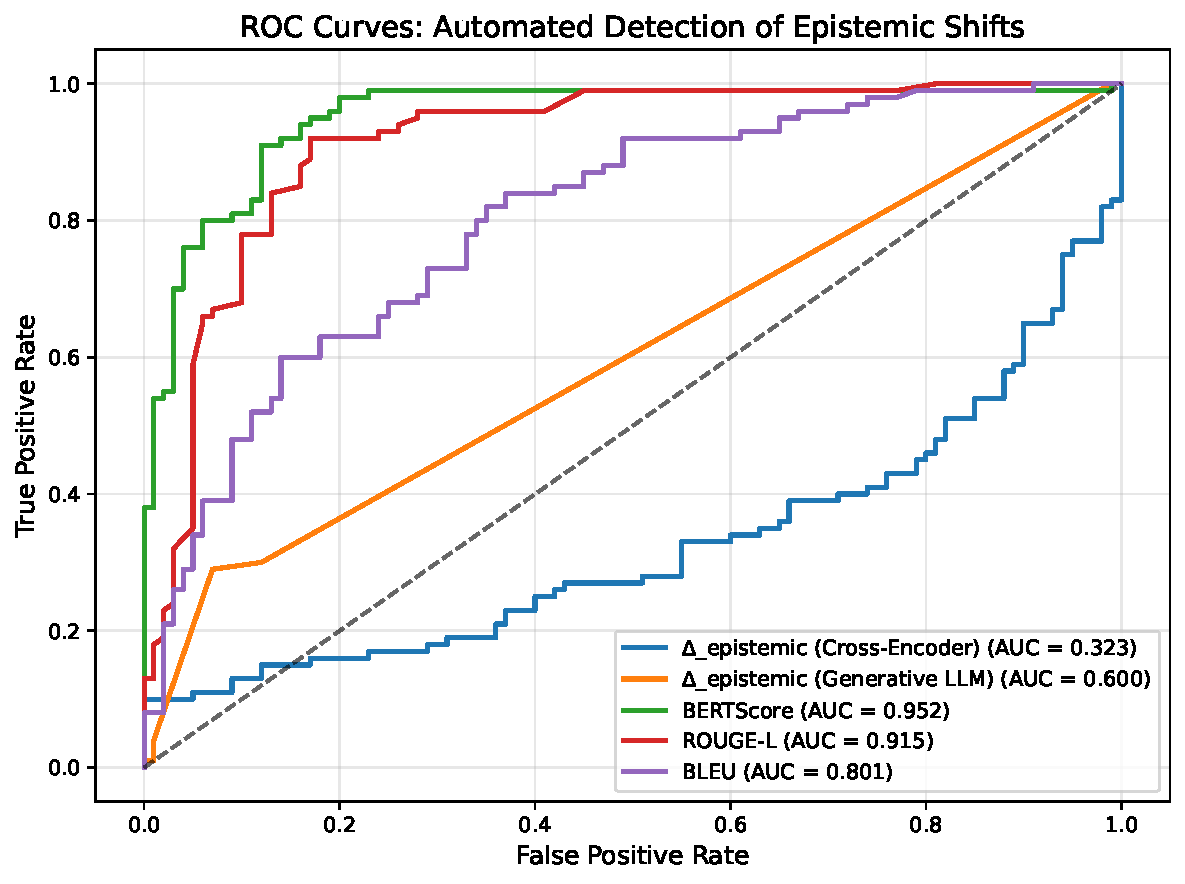
\includegraphics[width=0.85\linewidth]{publication_ROC_curves.pdf}
\caption{ROC Curves for Automated Detection of Epistemic Shifts. BERTScore provides highly reliable signal separation, while both NLI architectures (Cross-Encoder and Generative LLM) struggle significantly.}
\label{fig:roc}
\end{figure}

\subsection{The Collapse of General-Domain NLI}

As a baseline check bridging our work to prior methods, an initial zero-shot discrete classification test using \texttt{facebook/bart-large-mnli} failed to detect the causal escalation in 50\% of a 10-pair diagnostic subset, assigning identical labels to both versions of the dense biomedical text. 

When evaluating our continuous divergence metric, diagnostic probing revealed that the cross-encoder assigned an extremely low forward entailment probability ($\sim0.0003$) when evaluating if a causal premise (e.g., 'causes') entails a correlational hypothesis (e.g., 'associated with') destroying the asymmetrical $\Delta$ calculation. The Kernel Density Estimation (KDE) plot shows clearly that the $\Delta_{\text{epistemic}}$ scores for both the control and test pairs has reduced to one peak around zero (see Figure \ref{fig:kde_base}). This is because the models have been pre-trained on general MNLI/SNLI corpora so will be biased to think that any primary verb replacements are explicit contradictions rather than set-theoretic subset relations. This completely reduces the $\Delta$.

\begin{figure}[htbp]
\centering
\includegraphics[width=0.75\linewidth]{results/Figures/KDE_Distribution.png}
\caption{KDE Distribution for the Cross-Encoder ($\Delta_{\text{epistemic}}$). The extreme density overlap at 0.0 illustrates the model's complete inability to register localized causal escalation within dense biomedical contexts.}
\label{fig:kde_base}
\end{figure}

\subsection{Impact of Targeted Generative Modification}

Replacing the implicit cross-encoder with an explicit generative LLM using taxonomic rules (Pathway C) almost doubled the detection power of the metric (AUC=0.6002 compared to 0.3234). However, the 1.5B parameter LLM was still very far off the performance of BERTScore. 

Figure \ref{fig:kde_llm} illustrates the KDE distribution produced by this modification. The LLM produces a far more complex and multimodal distribution compared to the collapsed cross-encoder. Whilst some of the increased density is shifted to the right, upon qualitative error analysis we saw two distinct failure modes of the light-weight generative models:

\begin{itemize}
    \item \textbf{Context Overload (False Negatives):} In extremely dense biomedical sentences, the LLM failed to pick-up explicit causal escalations. The attention mechanism focused on the abundance of token similarities (often $>95\%$) rather than localised logical jumps, causing many values in the Test group to congregate around 0.0.
    \item \textbf{Synonym Hallucination (False Positives):} The generative model struggled to adapt to semantic changes. This can be seen in the peaks around 0.5 and 0.9 in the control (paraphrase) group of Figure \ref{fig:kde_llm}. Here, the model incorrectly awarded high escalation scores to safe semantic changes (e.g., ``associated with'' being misinterpreted as ``correlated with''), causing it to be labelled as an escalation due to the lack of strict adherence to the hardcoded taxonomy in the prompt.
\end{itemize}

\begin{figure}[htbp]
\centering
\includegraphics[width=0.75\linewidth]{results/Figures/KDE_Distribution_LLM.png}
\caption{KDE Distribution for the Generative LLM Modification. While multimodal, the model suffers from severe synonym hallucination, generating false-positive density peaks near 0.5 and 0.9 for the control paraphrase group.}
\label{fig:kde_llm}
\end{figure}

\section{Limitations and Future Directions}

We evaluate our experiments using a restricted synthetic dataset where there are only single-verb correlational-to-causal escalations under fixed context. In real applications, multiple edits involving complex multi-clause syntactic structures are often made when using an LLM. Deep semantic similarity metrics like BERTScore may struggle to separate acceptable large-scale syntactic paraphrases from targeted epistemic escalations. Future work is needed in order to perform such evaluations using real human authoring data (e.g. EarlySciRev). We also note that future LLM training will likely require causal-aware Reinforcement Learning (RLVR) to enforce true causal structures within the base models.

\section{Conclusion}

This work uncovers key limitations to utilising NLI models for auditing causal escalation in biomedical text. We show that explicit epistemic overclaiming (measured using either a cross-encoder model trained on general domain data or a generative LLM with explicit rules) is not possible due to context saturation, over-specificity and parameter driven overwrites. However, the semantic similarity between contextualised embeddings (as determined using BERTScore) naturally accounts for the subtle negative impacts of unwarranted causal escalation under fixed context (AUC = 0.9518). Using geometric embedding distance for automated text edits provides a much safer metric compared to logical entailment without any knowledge of the text.

\bibliographystyle{ACM-Reference-Format}
\bibliography{references}

\end{document}